\documentclass[a4paper,11pt]{report}
%
%--------------------   start of the 'preamble'
%
\usepackage{graphicx,amssymb}  %% ... with default font
\usepackage[slovene]{babel} % slovenski izpis naslovov in "c"s"z
\usepackage[latin2]{inputenc} % vnos 蹾 po ISO Latin 2
%\usepackage{graphicx,amssymb,mathptmx}  %%% times roman font
%\usepackage{graphicx,amssymb,mathpazo}   %%% another font
%\usepackage{graphicx,amssymb,newcent}   %%% another font
%\usepackage{graphicx,amssymb,cmbright}   %% yet another
%%%%%%%%%     more fonts in Chap 7 of the 'Companion'
%
%\newcommand\etc{\textsl{etc}}
%\newcommand\eg{\textsl{eg.}\ }
%\newcommand\etal{{\em et al.}}
%\newcommand\Quote[1]{\lq\textsl{#1}\rq}
%\newcommand\fr[2]{{\textstyle\frac{#1}{#2}}}
%
%---------------------   end of the 'preamble'
%
\begin{document}
%-----------------------------------------------------------
\title{JimmyIM - J2ME aplikacija za takoj�nje sporo�anje}
\author{\textbf{Avtorji (v abecednem vrstnem redu):}\\Matev� Jekovec (Jabber)\\Zoran Mesec (MSN)\\Dejan Sakel�ak (ICQ)\\Janez Urevc (uporabni�ki vmesik)}
\maketitle
%-----------------------------------------------------------
\begin{abstract}\centering
JimmyIM je J2ME aplikacija za takoj�nje sporo�anje. Podpira naslednje protokole:
Jabber, MSN in ICQ. Aplikacija je namenjena za uporabo na vseh mobilnih napravah,
ki podpirajo Javo\footnote{Java in J2ME sta za��iteni blagovni znamki podjetja
Sun Microsystems}.
\end{abstract}
%-----------------------------------------------------------
\tableofcontents
%-----------------------------------------------------------
\chapter{Uvod}
V zadnjem desetletju se je na podro�ju komunikacij
naredil ogromen korak. Razvoj telekomunikacij in
mobilnih naprav nam je omogo�il danes poleg prenosa govora
tudi po�iljanje in sprejemanje sporo�il, prenos ve�predstavnostnih
vsebin, integrirano navigacijo in podobno. Na podro�ju osebnih ra�unalnikov
pa je poleg elektronske po�te zacvetelo t.i. neposredno sporo�anje (eng. instant messaging).

Na�a seminarska naloga je vklju�evala razvoj aplikacije za mobilne telefone
za takoj�nje sporo�anje. Ker je dana�njih najbolj uporabljenih protokolov
za sporo�anje ve�, je bilo smiselno ustvariti aplikacijo, ki podpira ve�
protokolov hkrati. Uspe�no smo implementirali protokole Jabber, MSN in ICQ.
Aplikacijo smo napisali za mobilne naprave, ki imajo name��eno J2ME. Danes je
to �e ve�ina vseh mobilnih telefonov mlaj�ih od petih let.

\section{Razvojno okolje}
Za razvoj na�e aplikacije smo uporabili okolje Java 2 Mobile Edition
(http://java.sun.com/j2me). Podrejali smo se MIDP 2.0 in CLDC 1.1 standardom za mobilne naprave.
Kot IDE smo uporabljali Eclipse (http://www.eclipse.org) in NetBeans (http://www.netbeans.org).
Projekt je odprt in se nahaja na Berlios stre�niku
(http://developer.berlios.de/projects/jimmyim). Vsa izvorna koda in njena zgodovina se lahko dostopa
preko SVN drevesa (http://svn.berlios.de/wsvn/jimmyim).
Aplikacijo smo uspe�no testirali na telefonih:
\begin{itemize}
\item Siemens M65
\item Nokia 3220
\item Nokia 6610
\end{itemize}

\section{Pojmi}
Takoj�nje oz. neposredno sporo�anje je izraz za Instant messaging oz. IM v angle��ini.

JimmyIM (uradno ime), JIMMY (tehni�no ime), Jimmy (ime razreda) ali jimmy (ime paketa) so izrazi za ime na�e aplikacije za takoj�nje
 sporo�anje.
Razvijalec je v tej dokumentaciji mi�ljen programer, ki razvija aplikacijo.

Uporabnik je v tej dokumentaciji mi�ljen kot kon�ni uporabnik aplikacije na mobilnih telefonih.

\section{Licenca}
JimmyIM je last izklju�no njegovih avtorjev navedenih v datoteki AUTHORS in na
naslovnici tega poro�ila. Celoten projekt je odprt. Raz�irja se lahko pod pogoji
licence GNU GPL v2 (http://www.gnu.org/licenses/gpl.txt).

Slike protokolov (Jabber �arnica, MSN metulj in ICQ cvet) so last KDE programa
za neposredno sporo�anje, Kopete (http://kopete.kde.org).
\chapter{Osnovni razredi}
JimmyIM je razbit na ve� paketov:

\begin{itemize}
\item \textbf {jimmy}: Temeljni razredi, Ra�uni, Kontakti
\item \textbf {jimmy.net}: Razredi namenjeni povezovanju na IM stre�nike.
\item \textbf {jimmy.util}: Splo�ni algoritmi potrebni za komunikacijo z IM stre�niki (npr. MD5)
\item \textbf {jimmy.ui}: Uporabni�ki vmesnik
\item \textbf {jimmy.jabber}: Jabber protokol
\item \textbf {jimmy.msn}: MSN protokol
\item \textbf {jimmy.icq}: ICQ protokol
\end{itemize}

\section{Ra�uni}
\textbf{jimmy.Account}
Razred je namenjen hranjenju lastnosti ra�una. Podprti ra�uni:
\begin{itemize}
\item Jabber
\item MSN
\item ICQ
\end{itemize}

Vsak ra�un vsebuje naslednje lastnosti:
\begin{itemize}
\item Uporabni�ko ime (userName\_)
\item Geslo (password\_)
\item Ciljni stre�nik (po �elji) (server\_)
\item Ciljna vrata (po �elji) (port\_)
\item Samodejna prijava (autoLogin\_)
\end{itemize}

\section{Protokoli}
\textbf{jimmy.Protocol}
Vsak ra�un potrebuje za delovanje uporabo razreda Protocol. Abstraktni razred Protocol je v splo�nem namenjen prijavi, po�iljanju in sprejemanju sporo�il in stanj uporabnikov, odjavi, enkripciji ipd.

Glavne metode:
\begin{itemize}
\item constructor(Jimmy)
\item boolean login(Account)
\item void sendMsg(String)
\item void logout()
\end{itemize}

Implementacije abstraktnega razreda Protocol:
\begin{itemize}
\item JabberProtocol
\item MSNProtocol
\item ICQProtocol
\end{itemize}

Ve� o posameznih zna�ilnostih protokolov v poglavju Protokoli.

\section{Kontakti}
\textbf{jimmy.Contact}
Razred je namenjen hranjenju lastnosti kontakta. Kontakt je vsak uporabnik nekega protokola s katerim lahko komuniciramo. Kontakt vsebuje naslednje lastnosti:
\begin{itemize}
\item Uporabni�ko ime za doti�en protokol (userID\_)
\item Prikazano ime (screenName\_)
\item Stanje - na voljo, zaposlen, stran od ra�unalnika, nepovezan (status\_)
\item Ime skupine (groupName\_)
\item Referenca na protokol h katermu pripada (protocol\_)
\end{itemize}

\chapter{Opis protokolov}
\section{Jabber--XMPP}
\subsection{Splo�no}
Jabber (http://www.jabber.org) je najbolj raz�irjen odprt protokol za neposredno 
sporo�anje. Temelji na XML sintaksi. Osnovni, jedrni del je dokaj enostaven z obilico 
prostora za raz�iritve. Trenutno �e obstaja veliko odjemalcev (MirandaIM za Windows, 
Kopete za KDE, Gaim napisan v gtk+, deluje pod veliko OS, Bombus za J2ME in mnogi drugi), 
kot tudi stre�nikov (najbolj znan je v Javi napisan Wildfire). Ravno v tem �asu tudi 
Google razvija svoj Google Talk, ki uporablja XMPP kot temeljno sintakso za neposredno 
sporo�anje, za prenos zvoka pa odprt algoritem Speex (http://www.speex.org), vgnezden v XMPP 
sintakso. Naj omenim, da tudi danes najbolj popularen program za pogovor preko interneta, 
Skype (http://www.skype.org), uporablja Speex algoritem za kompresijo zvoka. Problem je le 
v zaprtosti protokola, saj je Skype lastni�ki komercialni program. Upajmo, da bo Googleova 
tradicionalna naklonjenost odprtokodni skupnosti tudi tokrat obrodila sadove.

Prav odprtost in enostavnost dajeta Jabberju prednost pred ostalimi protokoli. Jabber 
ni centraliziran, ampak obstaja celotna mre�a med seboj povezanih razli�nih stre�nikov 
(npr. jabber.org, gristle.org, predoslje.org). Vsak uporabnik ima svoje unikatno ime v 
obliki ime@stre�nik.

Jabber prav tako podpira razli�no enkripcijo pri prenosu sporo�il. Poleg standardne SASL 
in TLS povezave je na voljo tudi vi�jenivojska mo�na SHA1 (temelje�a na klju�ih oz. 
certifikatih) enkripcija podatkovenga dela XML kitice. Enkriptirani podatki se prena�ajo med 
odjemalcem in stre�nikom, kot tudi med stre�niki.

Prav tako zanimiva lastnost Jabber stre�nikov je t.i. prehod (gateway) med Jabberjem in 
ostalimi protokoli, torej da pretvorbo sporo�il in stanj uporabnikov v druge protokole 
izvaja Jabber stre�nik samodejno (npr. za Wildfire obstaja kopica raz�iritev za razli�ne 
protokole). Odjemalec mora poznati le Jabber sintakso.

\subsection{Zna�ilnosti}
\begin{itemize}
\item odprt protokol, jasna specifikacija
\item XML sintaksa
\item mo�na enkripcija celotno pot od odjemalca do odjemalca
\item hranjenje sporo�il na stre�niku, �e uporabnik trenutno ni dosegljiv
\item mo�nost raz�iritev obstoje�e sintakse na druga podro�ja (npr. VoIP)
\item konferen�na povezava
\item prenos datotek
\end{itemize}

\subsection{Implementacija}

\textbf{jimmy.jabber.JabberProtocol}

Osnovni razred, ki predstavlja protokol Jabber, je JabberProtocol. Po inicializaciji objekta 
pokli�e razvijalec metodo login(), ki aktivira nit (ki ves �as preverja stanje prejetih 
Jabber sporo�il na prihajajo�ih vratih), metoda pa vrne true ob uspe�ni prijavi ali false ob napaki. JabberProtocol 
se privzeto prijavi na stre�nik, ki je podan ob uporabni�kem imenu. Izjemoma se lahko uporabnik pove�e tudi na poljuben stre�nik,
�e ga poda ob ustvarjanju ra�una. Za po�iljanje sporo�il se uporablja standardna metoda sendMsg(), za odjavo pa logout().

JabberProtocol ne uporablja splo�nega DOM ali SAX raz�lenjevalnika (eng. parser), 
ampak smo zaradi hitrosti in optimizacije kode napisali specifi�ni raz�lenjevalnik, 
razred JabberParseXML, namenjen prav branju sporo�il, stanja kontaktov, spreminjanju 
lastnosti itd. za XMPP protokol.

JabberProtocol ne podpira �e nobene enkripcije linije, kot tudi ne enkripcije XML kitic. 
Vsi podatki se prena�ajo v �istem tekstovnem na�inu v UTF-8 kodnem naboru.

\subsection{Podprte zna�ilnosti}
\begin{itemize}
\item podpora ve�ih Jabber ra�unov hkrati
\item za�etek pogovora s poljubnim kontaktom na poljubnem Jabber stre�niku, �e je pobudnik pogovora uporabnik
\item za�etek pogovora s poljubnim kontaktom na poljubnem Jabber stre�niku, �e je kontakt pobudnik pogovora
\item prikaz stanj kontaktov (online, offline, busy, away)
\item urejanje lastnosti kontakta in dodeljevanje skupinam
\item dodajanje kontaktov, �e je pobudnik JIMMY uporabnik
\item dodajanje kontaktov, �e je pobudnik kontakt
\item brisanje kontaktov
\end{itemize}

\section {MSNP}
\subsection {Splosno}

MSN Messenger je program za neposredno sporo�anje, sicer produkt podjetja Microsoft. 
Na trgu je vse od leta 1999, od takrat je do�ivel veliko izbolj�av in pohitritev. 
Program sodi med �tiri najpriljubljenej�e programe za neposredno sporo�anje, najbr� lahko re�emo, 
da je med slovenskimi uporabniki kar najpogostej�i. Razlog, da smo v Jimmy-iju implementirali 
MSN protokol je pogostost uporabe med slovenskimi uporabniki. Program  MSN Messenger je bil 
izhodi��e za implementacijo MSN protokola na Jimmy-ju. Sorodnosti med funkcionalnostjo obeh 
programov so o�itne, mo�no je opaziti tudi podobnosti z drugimi protokoli in programi za 
neposredno sporo�anje. 

Program za komunikacijo uporablja tekstovni protokol, ki se imenuje MSN Messenger protokol 
(z angle�ko kratico MSNP). Protokol je tekstovni in ni enkriptiran. 
Osnovni namen protokola je neposredno sporo�anje. Uporabniki med seboj 
delijo in si posredujejo podatke o prisotnosti, datoteke in sporo�ila.  
Obstaja tudi http razli�ica, vendar te nismo implementirali zaradi omejenih 
resursov na mobilnih telefonih. Protokol je centraliziran - naloge opravlja centralni stre�nik. 
Vsaka menjava informacije med razli�nimi odjemalci, poteka preko centralnega stre�nika, 
mimo te povezave sporo�anje med uporabniki ni mo�no. Med delovanjem bo torej na� program 
``govoril'' oz. po�iljal informacije do centralnega stre�nika, ki bo nato poskrbel, 
da paketi pridejo do pravega naslovnika. Kakorkoli �e, obstajajo tudi dolo�eni ukazi 
protokola za katere velja, da jih centralni stre�nik ne obdela, temve� samo posreduje 
do naslovnika - ukazi se nato procesirajo pri naslovniku (o tak�nih ukazih ve� kasneje).  

Microsoft je bil precej skop glede informacij o protokolu. Dokumentacijo so napisali 
samostojni razvijalci  s pomo�jo t.i. ``reverse engineeringa''. Zaradi pomankljive 
dokumentacije je programiranje odjemalcev MSN protokola postalo te�avno in zdi se, da 
so nekatere spremembe nastale zato, da bi odvrnili samostojne razvijalce od razvijanja 
tak�nih odjemalcev. To sovpada s politiko podjetja Microsoft, ki �eli od uporabnikov, da 
v �imve�jem �tevilu uporabljajo njihove produkte(v tem primeru program MSN Messenger) in 
seveda operacijski sistem MS Windows. Toda kot bodo�i ra�unalni�ki in�enirji moramo tak�ne
 poteze grajati. Potreba po standardizaciji tako na internetu kot na podro�ju programske opreme 
 je danes zaradi porasta razli�nih tehnologij, ki temeljijo na razli�nih jedrih, nujnej�a kot 
 kdajkoli prej in za�eleno je, da so proizvodi odprte narave (bodisi odprtokodni ali pa potrjeni 
 od organizacij za standardizacijo kot je npr. ISO), ravno zaradi prenosljivosti in dostopnosti. 
 Nasploh je zadnja leta v ra�unalni�tvu �utiti tendenco po ve� platformnih re�itvah in resno 
 konkurenco odprto-kodnih re�itve prav zaradi la�je dostopnosti in prenosljivosti. Tu naj 
 ponovno omenim, da je bila dokumentacija za MSN protokol, ki je dostopna �ir�i javnosti, 
 spisana s pomo�jo t.i. ``reverse engineering-a''. To dejstvo dokazuje moje trditve, da �eli 
 Microsoft odvrniti ostale razvijalce programske opreme od uporabe MSN protokola. 
 
 
\subsection{Zna�ilnosti}
\begin{itemize}
\item ozaprt protokol, pomankljiva specifikacija
\item specifi�na sintaksa
\item ni enkripcije
\item hbrez raziritve sintakse
\item konferen�na povezava
\item prenos datotek
\end{itemize}

\subsection{Implementacija}

\textbf{jimmy.msn.MSNProtocol}

Osnova za implementacijo je razred MSNProtocol.java, ki podeduje abstraktni razred Protocol.java. Za pravilno delovanje so potrebni �e ostali razredi:
\begin{itemize}
  \item \textbf{MSNTransaction:} skrbi za pravilno obliko otevil�enje sporo�il
  \item \textbf{PassportNexus:} avtentifikacija in pridobivanje vstopnega zaporedja
\end{itemize}

Najve� te�av povzro�a nepredvidljiva oblika ukazov, ki imajo lahko spremenljivo tevilo parametrov in pomankljiva oziroma zastarana dokumentacija. Z vsako verzijo protokola se sintaksa malenkostno spremeni, kar ote�uje sledenje razvijalcev. 
	Dale� najte�ja zadeva je algoritem za t.i. ``challenge'' ali izziv. Centralni stre�nik namre� takoj po prijavi polje ukaz CHL(npr. ``CHL 0 26045552712758918823''), na katerega je treba pravilno odgovoriti v roku ene minute, sicer stre�nik odjemalca odjavi iz sistema. Prvotni na�rt implementacije je bila enajsta verzija protokola, toda izkazalo se je, da ima ta verzija veliko te�avneji challenge algoritem kot predhodne verzije, zato smo naknadno izbrali deveto oziroma deseto verzijo protokola. Challenge algoritem za omenjeni verziji sedaj obsega MD5 predstavitev 16 mestnega parametra v stre�nikovem ukazu. �etudi se sli�i enostavno, je implementacija v okolju j2me dokaj zapletena zaradi omejenih funkcionalnosti.

\subsection{Od prijave do sporo�anja}

	Seja MSN protokola poteka vsebuje najprej povezavo z t.i. ``Notification serverjem'', ki posreduje podatke o prisotnosti. Notification server dovoljuje uporabniku, da se pove�e na Switchboard stre�nik, ki  opravlja zahteve neposrednega sporo�anja.

Centralni stre�nik je dosegljiv na naslovu messenger.hotmail.com, port 1863. Med klientom in ste�nikom se najprej izmenja informacija o verziji protokola in verziji klienta (ukazi VER, CVR) in povezava se nato zaklju�i. Prijava v MSN omre�je poteka na drugem preko t.i. Notification server(kraje NS) na druga�nem IP naslovu - obi�ajno baym-cs118.msgr.hotmail.com, kjer se najprej ponovi izmenjava ukazov s centralnega stre�nika. NS kasneje opravlja vse ostale ukaze, zato je dale� najve� komunikacije opravljene prav na tej relaciji. Potrebno je omeniti, da je med procesom prijave, potrebno vzpostaviti varno povezavo(HTTPS) do t.i. Passport Nexus(PN) stre�nika in tja posredovati up. ime  in geslo. PN nato vrne napako ali pa dolg niz znakov ob uspehu. Ta niz znakov predstavlja dovoljenje, ki ga nato  uporabimo pri NS stre�niku za kon�ni proces prijave. NS takoj zatem polje podatke o prisotnosti kontaktov z ukazoma LSG in LST.
	Sporo�anje oz. pogovor med dvema uporabnikoma poteka tako, da pobudnik od NS zahteva pogovor z ukazom XFR. NS nato ustvari kanal za sporo�anje na nekem IP naslovu in ta naslov sporo�i. Uporabnik nato vzpostavi povezavo na ta kanal in povabi prijatelje s katerimi �eli klepetati z ukazom CAL(najbr� to pomeni call - klicanje). Klicani nato odgovori z ukazom JOI, kar pomeni join ali priklju�il sem se pogovoru. Na kanalu se nato prenaajo sporo�ila z ukazi MSG. Mo�no je seveda na kanal povabiti tudi ve� prijateljev z ukazi CAL in tako ustvariti konferen�no zvezo.

\subsection{Format ukazov}

Sintaksa je na pogled preprosta, toda kasneje se izka�e, da obstaja mnogo razli�nih variacij istega ukaza (npr. razli�no tevilo parametrov), kar mo�no ote�uje implementacijo. Sintaksa je slede�a:

\begin{quote}
UKZ stTr (par1 par2 par3 ...)$\backslash r \backslash n$
\end{quote}

\begin{itemize}
  \item UKZ - vrsta ukaza
  \item stTr - transakcijska tevilka, ki se pove�a za 1 po vsakem prenosu
  \item (par1 par2 par3 ...) - parametri in podatki, lo�eni s presledki
  \item na koncu sta vedno znaka carriage return in newline
\end{itemize}

\subsection{Nabor najpogostejih ukazov:}

\begin{itemize}
\item za�etna predstavljanje:
  \begin{itemize}
  \item VER: verzija protokola (npr. ``VER 1 MSNP11 MSNP10 CVR0$\backslash r \backslash n$'')
  \item CVR: podatki o klientu(verzija, naziv), operacijskem sistemu in ra�unalniki arhitekturi uporabnika
  \end{itemize}

\item za�etna avtentifikacija:
  \begin{itemize}
  \item USR: podatki uporabnika(uporabniko ime, geslo)
  \end{itemize}

\item podatki o prisotnosti:
  \begin{itemize}
  \item LSG: podatki o skupinah. Vsaka skupina predstavlja eno LSG sporo�ilo. Npr.: LSG Ime skupine 124153dc-a695-4f6c-93e8-8e07c9775251$\backslash r \backslash n$
  \item LST: podatki o kontaktih. Podobno kot pri skupinah, vsak kontakt je predstavljen v enem sklopu LST, znotraj je tudi skupina kateri pripada.
  \end{itemize}
  

\item sporo�anje:
  \begin{itemize}
  \item MSG: ozna�uje prenos sporo�ila. Vsebuje informacije o pisavi, MIME tipu in vsebini.
  \end{itemize}

\end{itemize} 
Primer takega sporo�ila z MSG ukazom:
\begin{quote}
MSG 4 N 133$\backslash r \backslash n$
MIME-Version: 1.0$\backslash r \backslash n$
Content-Type: text/plain; charset=UTF-8$\backslash r \backslash n$
X-MMS-IM-Format: FN=Arial; EF=I; CO=0; CS=0; PF=22$\backslash r \backslash n$ $\backslash r \backslash n$

Pozdravljeni! Kako ste?
\end{quote}

\subsection{Podprte zna�ilnosti}
\begin{itemize}
\item podpora ve�ih MSN ra�unov hkrati
\item prikaz stanj kontaktov (online, offline, busy, away)
\item za�etek pogovora s poljubnim kontaktom
\item dodajanje kontaktov, �e je pobudnik JIMMY uporabnik
\item dodajanje kontaktov, �e je pobudnik kontakt
\item brisanje kontaktov
\end{itemize}

\section{ICQ}
\subsection{Protokol (OSCAR) in implementacija}
OSCAR (Open System for CommunicAtion in Realtime) je binarni protokol za instantno sporocanje,
ki je leta 2001 nadomestil takratni ICQ-jev TOC protokol. Neglede na njegovo ime, je protokol
zaprt in specifikacijo si lasti AOL. Do ``odprtih'' in nenatan�nih specifikacij protokola
so se nekateri prebili z obratnim in�eniringom. OSCAR se trenutno uporablja za ICQ in AIM
komunikacijska sistema. Sistema uporabljata skupni nabor enot protokola, a vsak od njiju
ima tudi entitete, ki niso skupne obema.

Komunikacija med stre�nikom in odjemalcem poteka v paketni obliki. OSCAR vsebuje tri nivoje
paketov in sicer FLAP, SNAC in TLV. Pogosto se v FLAP ali SNAC paketu nahajajo tudi goli
podatki, ki niso v paketni obliki.

\begin{enumerate}
\item FLAP: Osnovni nivo, preko katerega se prena�ajo vsi podatki. Vsebuje informacijo
  o kanalu (tipu podatkov, v njemu), dol�ini podatkov, zaporedno �tevilko paketa ter podatke.
  \begin{enumerate}
  \item Kanal 1 -- ``Hello'': Namenjen je osnovni avtentifikaciji.
  \item Kanal 2 -- ``SNAC'': Samo preko tega kanala se prena�ajo SNAC "paketi".
  \item Kanal 3 -- ``Error'': Ko se prejme nepravilen paket oz. pride do napake
    na FLAP nivoju, se odjemalcu/stre�niku po�lje informacija o napaki preko tega kanala.
  \item Kanal 4 -- ``Disconnect'': Ko prejmemo paket s tem kanalom, moramo prekiniti povezavo.
  \item Kanal 5 -- ``Keepalive'': Da stre�niku vedeti, da je odjemalec �e vedno �iv.
  \end{enumerate}
\item SNAC: Storitveni nivo, ki natan�neje definira vsebino paketa. V glavi je zabele�ena
dru�ina stortve, ukaz, zastavice ter referenca zahtevka. Poznanih je pribli�no 23 dru�in
storitev, od katerih ICQ uporablja pribli�no polovico.
\item TLV: Ime tega nivoja je kratica za ``Type Length Value'' , kar nam pri�epne, da so v
teh paketih dejanski podatki. V glavi paketa je zapisano ime podatka ter njegova dol�ina.
\end{enumerate}

\begin{figure}[h]
\centering
 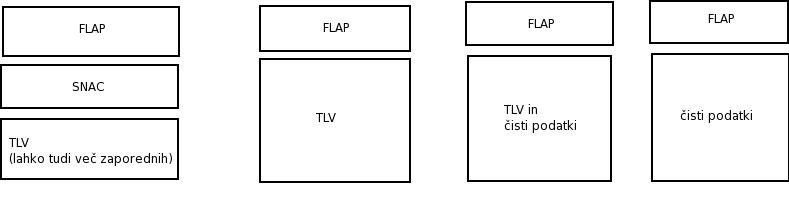
\includegraphics[width=.7\textwidth]{icq_oblike_paketov.jpg}
 \caption{Sestava paketov}
 \label{fig:pic}
\end{figure}

Storitev, ki so mo�ne v ICQ sistemu je veliko. Od obi�ajnega pogovarjanja in sledenja
kontaktom do reklam itd.

Prijava za vse AOL-ove storitve poteka preko avtentifikacijskega stre�nika, ki odjemalcu dodeli
``pi�kotek'' z osnovnimi informacijami. S pomo�jo tega pi�kotka se je mo�no prijaviti na vse
AOL-ove storitve (ICQ, AIM, reklamne storitve, ...). Pi�kotek prejmemo po �etrtem kanalu, kar pomeni,
da je avtentifikacija odjemalca/uporabnika kon�ana. Poleg pi�kotka je v istem paketu tudi naslov
BOS (Basic OSCAR Service), na katerega se pove�emo v naslednjem koraku. BOS stre�niku najprej
po�ljemo prej sprejeti pi�kotek, nato se za�ne izmenjava osnovnih informacij, kot so varnostne
omejitve po�iljanja dolo�enih skupin paketov, podprte storitve, SSI (Server Side Information) in
seznam kontaktov. Ko se vsi podatki izmenjajo, po�lje odjemalec stre�niku ``OK'' paket, ki stre�niku in
vsem kontaktom sporo�i on-line status. Jimmy po tem koraku po�ene lastno nit in po�lje �e dolo�ene
pakete za obve��anje o spremembi statusa kontaktov. Ponavadi se v tem trenutku po�lje tudi zahtevek
po ``off-line'' sporo�ilih, ki so se v �asu odsotnosti shranila na stre�niku, a �al ta funkcija
ni vklopljena v Jimmyju zaradi var�evanja prenosov. Opisan postopek prijave trenutno ni popolnoma
dinami�en in potrebuje �e nekaj popravkov. Problemi se pojavijo, ko stre�nik onemogo�i povezavo,
uporabimo napa�no ime in geslo ali pride do kake napake (popravljeno bo v kon�ni razli�ici).

\begin{figure}[h]
\centering
 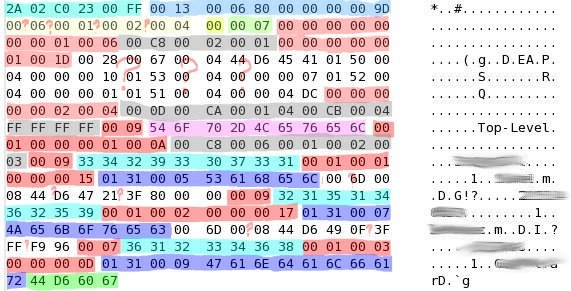
\includegraphics[width=.7\textwidth]{icq_paket.jpg}
 \caption{Primer paketa (Seznam kontaktov)}
 \label{fig:pic}
\end{figure}

Nadaljnji del implementacije poteka v zanki, ki se kon�a ob odjavi. Vsak zankin cikel se preberejo
nove vrednosti iz bralnega izravnalnika toka podatkov povezave. Sprejete podatke se razre�e na pakete,
ki jih tolma�imo in s pomo�jo njihovih ukazov izvedemo akcijo (po�ljemo sporo�ilo jedru, nastavimo
nov status kontakta itd.).

Paketi v sistem pridejo v obliki tabele bajtov ter se pretvorijo v objekte, na katerih so
definirane dolo�ene operacije. Po pretvarjanju (rezanju glav paketov) se paket tolma�i.
Tolma� pakete spu��a skozi switch stavek. Ko se ujame, se iz njega izvle�ejo podatki in
glede na njih nato izvede pripadajo�o akcijo.

Po�iljanje paketov izgleda podobno, le da v ve�ini primerov njihovo po�iljanje povzro�i
klic metode iz Jimmyjevega jedra. Paket se pripravi z generiranjem novega osnovnega paketa.
�e bo paket vseboval SNAC podatke, bo potrebno nastaviti tudi parametre SNAC glave. Ker je
vsebina paketa lahko zelo razli�na, je potrebno tudi to nastaviti po dolo�enem postopku.
Podatke, ki so ``prosto plavajo�i'' , se nastavi kot vsebino v obliki tabele bajtov. �e �elimo
pripeti tudi TLV paket, moramo ustvariti nov TLV objekt in mu nastaviti vse koli�ine ter ga
dodati v seznam TLV paketov v na�em osnovnem paketu. Ko so vsi podatki v njem, se pokli�e
metodo, ki vrne paket v tabeli bajtov in jo po�lje v tok.

Implementacija protokola je za na� primer omejena samo na ICQ sistem. Razporejena je �ez ve�
javinih razredov: {\it Protocol}, {\it ICQProtocol}, {\it ICQPackage}, {\it ICQTlv}, {\it ServerHandler}, {\it ICQConnector},
{\it ICQContact}, {\it Utils} ter ostale razrede za interakcijo z jedrom. {\it ICQProtocol} je raz�iritev
abstraktnega razreda {\it Protocol}, ki je gradnik implementacij vseh protokolov v Jimmyju in vsebuje
poleg osnovega nabora atributov ter metod �e dolo�ene, za ICQ specifi�ne, kot so metode za
tolma�enje, metode za spreminjanje stanj v instanci ter metode za branje vrednosti iz jedra.
{\it ICQPackage} je splo�na specifi�na podatkovna struktura, ki ima definirane operacije zase.
Vsebuje dolo�ene zbirke ter metode za vra�anje vsebine in nastavljanje vsebine. {\it ICQTlv} je
namenjena generiranju TLV paketov. Definirana je sama zase, da lahko iz nje naredimo ve� instanc.
Vsebuje operacije ter strukture nad katerimi izvajamo te operacije. {\it ICQConnector} je raz�iritev
{\it ServerHandler} razreda, ki omogo�a enostavnej�e branje paketov. {\it ServerHandler} namre� vra�a
vse, kar se je spravilo v bralni medpomnilnik, kar pa se lahko odra�a v ve�jem �tevilu FLAP
paketov. S klicem metode za vra�anje paketa v {\it ICQConnectorju} tako to informacijo razre�emo
na pakete in shranimo v zbirki ter ob vsakem ciklu zanke preverimo �tevilo paketov v njej
ali preberemo novo iz medpomnilnika. {\it ICQContact} je samo raz�iritev splo�nega razreda {\it Contact}.
Ima dodatna polja za hranjenje informacij o ID-ju skupine in samega kontakta v SSI
(Server Side Information) seznamu.

Ker so v OSCAR-ju vsi podatki v binarni obliki, potrebujemo pripomo�ke za pretvorbe med
razli�nimi tipi. V razredu Utils tako najdemo stati�ne metode za pretvarjanje iz tabel
bajtov v short, int ali long primitive ter obratno.

\subsection{Problemi}
Na poti do uspe�nega delovanja sem se sre�al z velikim �tevilom problemov, ki so bili �asovno
zelo po�re�ni. Problemi so sicer nastali zaradi pomanjkljive in nepopolne
dokumentacije protokola, a so v veliki meri nastale tudi zaradi slabega na�rtovanja le tega.

Najhuj�i problem je bil z razumevanjem prijavne sekvence, ker v nobeni dokumentaciji ni
pisalo kako to�no prijava izgleda. V dolo�enih dokumentacijah je bila prijava celo pretirano
napihnjena in zakomplicirana. Pri tem problemu so me re�ile �e narejene implementacije. Z
orodjem za bele�enje mre�nih paketov (ethereal) sem bele�il komunikacijo s stre�nikom in na
tak na�in nekako izsledil pravilna zaporedja. Ko sem pa �elel dolo�eno funkcionalnost
izklopiti zaradi omejitve na GSM aparatih, sem do�ivel tudi spremembo zaporedja, kar je
vplivalo tudi na motivacijo.

Problem je nastal tudi pri razumevanju vsebine paketa s kontaktno listo in skupinami, ker
sem zaradi druga�nega prijavnega zaporedja v njem dobil �e dolo�ene neznane podatke, ki so
mi podrli logiko.

Del, ki �e ni popolnoma implementiran, je dodajanje in odstranjevanje kontaktov, kajti v
nobeni dokumentaciji ne pi�e, kako se to po�ne, in je potrebno vse bele�iti in iskati izjeme
ter ugotavljati delovanje.

Sre�al sem se tudi s problemom pretvarjanja sprejetega besedila iz Unicode tabele bajtov v
Unicode besedilo. Tega problema �e nisem odpravil, bo pa nujno to realizirati, kajti nesmiselno
je sprejemanje dvojne koli�ine podatkov, �e potem ni mo\v zno izkoristiti prednosti, ki jih ta
oblika zapisa ponuja.

\subsection{Lastno mnenje}
Med implementacijo sem se velikokrat spra�eval, zakaj se je OSCAR razvil v tako obliko.
S primerjavo osnovne ideje paketne oblike s kon\v cno obliko sem ugotovil, da je protokol take
oblike zaradi posku\v sanja ohranitve njegove zaprte specifikacije. S kompliciranjem vsebine
paketov posku\v sa AOL omejiti \v sirjenje neuradnih odjemalcev. Ta pristop mo\v cno ote\v zuje
dekodiranje in razumevanje vsebine paketov ter pove\v cuje redundanco.

Sam protokol je bil v za\v cetku dobro zami\v sljen, a \v se vedno pre\v siroko, glede na njegovo
trenutno uporabo. Veliko podatkov, ki se po\v siljajo/sprejemajo vsebuje popolnoma odve\v cne
vrednosti v glavah paketov. SNAC glave vsebujejo prostor za definicijo ve\v c tiso\v c razli\v cnih
dru\v zin storitev, uporablja pa se jih zgolj 23 (podobno velja tudi za ukaze storitev).

Zmogljivost TLV nivoja je v OSCAR-ju popolnoma neizkori\v s\v cena, kajti v ve\v cini primerov
se uporablja kar plavajo\v ce podatke, kar pa TLV paketi omogo\v cajo sami po sebi z manj\v so
redundanco. TLV glava definira tip podatka, ki pa je tako kot ostale re\v ci v ve\v cini primerov
zanemarjena in neizkori\v scena.

Jimmy se bo v prihodnosti razvijal in izbolj\v seval iz generacije v generacijo. Implementacije
komunikacijskih protokolov se bodo spreminjale v bolj dinami\v cne ter hitrej\v se oblike. S
popravki uporabljene dokumentacije bom dosegel bolj\v so preglednost in razumljivost implementiranih
funkcionalnosti.

Kar se protokola ti�e, je bil v osnovi dobro zami�ljen, a pritisk trga je z njim odigral grdo
igro z vrivanjem nepremi�ljenih funkcionalnosti. Povozili so ga tudi rivali, ki uporabljajo
novej�e principe kot je prenos informacije v obliki XML.

Protokol zaradi pre�iroke zasnove tako povzro�a velike redundance poslanih paketov. Veliko
�tevilo neuporabljenih atributov in nesmiselnih podatkov se na tak na�in prena�a preko mre�e.

\chapter{Uporabni�ki vmesnik}

\section{Uvod}
Izvorne datoteke razredov uporabni�kega vmesnika se nahajajo v podimeniku ./ui, 
kateri se nahaja v korenskem imeniku z izvorno kodo. Imenik vsebuje naslednje datoteke:

\begin{itemize}
\item JimmyUI.java -- v tej datoteki se nahaja razred, ki je osnova za komunikacijo med 
uporabni�kim vmesnikom in ostalimi deli aplikacije.  Ves pretok informacij med uporabni�kim 
vmesnikom in razredi, ki skrbijo za protokol, poteka preko tega razreda.
\item MainMenu.java -- izvorna koda okna, kjer lahko uporabnik dodaja, bri�e in spreminja 
podatke o ra�unih za razli�ne protokole. Poleg tega lahko uporabnik na tej strani 
spro�i vzpostavljanje ali prekinitev povezave,
\item NewAccount.java -- podokno, kjer uporabnik dolo�i podrobnosti (uporabni�ko ime, 
geslo, ...) za ustvarjanje novega ali spremembo obstoje�ega ra�una,
\item ContactsMenu.java -- okno, kjer se izpi�e seznam kontaktov za vse ra�une, ki so 
trenutno povezani. Kontakti so razdeljeni v skupine;
\item EditContact.java -- podokno, kjer uporabnik dodaja nove ali spreminja obstoje�e kontakte;
\item ChatWindow.java -- okno za komunikacijo z izbranim uporabnikom;
\item About.java -- okno s podatki o avtorjih in osnovnih informacijah o programu;
\item Splash.java -- pozdravno okno, ki se prika�e ob zagonu programa in med operacijami, ko 
je program zaseden
\end{itemize}

Razen razreda JimmyUI, so vsi izpeljani (extendani) iz razli�nih implementacoij razreda 
Displayable. Vsak objekt tega tipa se lahko samostojno prika�e na zaslonu naprave kot 
samostojno okno. Posamezne implementacije slu�ijo specifi�nim problemom. Programer lahko 
za vsako okno izbere podrazred, ki mu za realizacijo dolo�enega okna najbolj ustreza. Na 
voljo imamo forme, sezname, tekstovna okna ipd.

Posamezna okna v Jimmy-ju sem implementiral tako, da sem jih izpeljal iz najprimernej�ih 
razredov Javine knji�nice in jim dodal �eljene funkcionalnosti. Ob zagonu programa se 
celoten uporabni�ki vmesnik ustvari kot objekt tipa JimmyUI, preko katerega se posredno 
ustvarijo vsa okna in gumbe.

Objekt JimmyUI skrbi za pravilno interpretiranje ukazov in komunikacijo med protokoli in 
uporabni�kim vmesnikom. �e �eli protokol posredovati informacijo v uporabni�ki vmesnik, 
to stori s klicem ustrezne metode iz vmesnika ProtocolInteraction.

\section{Opis dogajanja ob zagonu programa}
Ob zagonu programa se na zaslonu najprej prika�e pozdravno okno, ki uporabnika med procesom 
zaganjanja obve��a o trenutnem dogajanju. Temu sledi branje podatkov o ra�unih in  nastavitev 
iz pomnilnika. Zaradi  narave implementacije pomnilnika se nato izvede optimizacija spomina. 
Java podatke  shranjuje kot seznam zapisov. Problem je v tem, da brisanje zapisa dejansko ne 
izbri�e, ampak samo ozna�i kot neuporabnega. Med optimizacijo zato celoten spomin izbri�emo 
in ponovno shranimo podatke o ra�unih in nastavitvah. S tem se uspe�no znebimo neuporabnih 
zapisov v pomnilniku.

Od tu naprej imamo ve� mo�nosti:
\begin{enumerate}
\item �e ne obstaja �e noben ra�un, se uporabniku odpre okno za kreiranje novega ra�una;
\item v kolikor noben od obstoje�ih ra�unov ne zahteva avtomati�ne prijave, se odpre okno s 
seznamom ustvarjenih ra�unov, kjer uporabnik izbere ra�un s katerim se �eli prijaviti;
\item v primeru, da kateri od ra�unov zahteva avtomati�no prijavo, se ta izvede. Po uspe�no 
izvedeni prijavi se uporabniku prika�e okno s seznamom knotaktov.
\end{enumerate}

\section{Opis posameznih modulov uporabni�kega vmesnika}

V tem poglavju bom vsak del vmesnika opisal bolj podrobno. Opisane podrobnosti se nana�ajo 
na uporabni�ki vmesnik, kakr�nega prika�e Sunov emulator za J2ME aplikacije. Zaradi narave 
Javinih knji�nic za uporabni�ki vmesnik lahko na razli�nih napravah pride do razlik v prikazu 
in razporeditvi ukazov na zaslonu.


\subsection{Okno s seznamom aktivnih ra�unov}
V tem oknu so prikazani ustvarjeni uporabni�ki ra�uni. Poleg uporabni�kega imena je prikazan 
tudi logotip protokola (sli�ice so last avtorjev KDE progama Kopete). Uporabnik lahko v meniju 
izbere naslednje ukaze:

\begin{itemize}
\item Login -- povzro�i prijavo trenutno izbranega ra�una. Med povezovanjem se prika�e 
pozdravno okno. �e je prijava uspe�na, se prika�e seznam kontaktov, v nasprotnem primeru 
pa je uporabnik o neuspehu obve��en. Isto�asno je lahko povezanih ve� re�unov;
\item Logout -- povzro�i odjavo trenutno izbranega ra�una. Poleg tega se iz seznama 
odstranijo vsi kontakti, ki so pripadali tej povezavi;
\item New -- odpre okno za ustvarjanje novega ra�una;
\item Edit -- odpre okno za spreminjanje nastavitev izbranega ra�una;
\item Delete -- izbri�e izbrani ra�un;
\item Back -- zapre okno in se vrne na seznam kontaktov
\end{itemize}

\subsection{Okno za dodajanje novega ra�una}
Okno vsebuje naslednja polja:
\begin{itemize}
\item seznam protokolov;
\item polje za uporabni�ko ime. Uporabni�ko ime se vnese v obliki uporabjnik@domena. Polje 
je obvezno.
\item polje za geslo. Geslo se med vna�anjem zamaskira z zvezdicami. Polje je obvezno;
\item polje za ime stre�nika. �e se ne uporablja privzeti, uporabnik sem vnese ime 
nadomestnega stre�nika. Polje ni obvezno;
\item polje za �tevilko vrat. Uporablja se samo, �e se ne uporaljajo standardna vrata. Polje 
ni obvezno
\item izbira avtomati�ne prijave ob zagonu;
\end{itemize}

S klikom na gumb OK, se ra�un shrani in prika�e na seznamu obstoje�ih ra�unov. Back povzro�i 
brisanje vne�enih parametrov in vra�anje na seznam ra�unov.


\subsection{Okno za sreminjanje nastavitev obstoje�ega ra�una}
Okno vsebuje naslednja polja:
\begin{itemize}
\item geslo;
\item ime dodatnega stre�nika;
\item vrata;
\item izbira avtomati�ne prijave ob zagonu;
\end{itemize}

Okno je zelo podobno tistemu za dodajanje novega ra�una. V posameznih poljih se nahajajo 
trenutno nastavljene vrednosti, ki jih uporabnik lahko spremeni. Spremembe se shranijo s 
klikom na OK, pobri�ejo pa s klikom na Back. V obeh primerih se ponovno prika�e okno s 
seznamom ra�unov.

\subsection{Okno s seznamom kontakotv}
V tem oknu se nahaja seznam kontaktov vseh trenutno povezanih ra�unov. Kontakti so 
razdeljeni v skupine. Poleg vsakega kontakta je prikazan logotip protokola, 
kateremu pripada. Logotip je �rno-bel, �e ima kontakt status ``odsoten'',  bodisi barven 
v vseh drugih primerih. Uporabnik lahko v meniju izbere naslednje ukaze:
\begin{itemize}
\item Chat -- s klikom na ta gumb se pri�ne nov pogovor (ali nadaljuje obstoje�) s trenutno 
izbranim kontaktom. �e je trenutlo izbrana labela z imenom skupine se ne zgodi ni�.
\item New contact -- klik na ta gumb odpre pogovorno okno za dodajanje kontakta.
\item Delete contact  - klik na ta gumb izbri�e trnutno izbran kontakt.
\item Edit -- odpre okno za spreminjanje skupine in psevdonima za trenutno izbran kontakt.
\item Accounts -- odpre meni s seznamom ra�unov.
\item About -- prika�e podatke o avtrojih in programu.
\item Exit -- povzor�i izhod iz programa. Med uga�anjem programa se prika�e pozdravno okno.
\end{itemize}

\subsection{Okno za dodajanje kontakta}
Okno ima naslednja polja:
\begin{itemize}
\item Protokol -- v tem pop-up meniju izberemo protokol, kateremu �elimo dodati kontakt.
\item uporabni�ko ime -- sem vpi�emo uporabni�ko ime kontakta (oblike: uporabnik@domena)
\item psevdonim -- psevdonim, pod katerim se bo kontakt prikazal v seznamu. �e je polje 
prazno se bo prikazalo kar uporabni�ko ime
\item skupina -- v tem pop-up meniju izberemo bodisi edo izmed obstoje�ih skupin, bodisi 
uporabniku ne dodelimo nobene skupne (``No group''), bodisi ustvarimo novo (``Other'')
\item nova skupina -- �e smo v meniju za izbiranje skupine izbrali ``Other'', tukaj vpi�emo 
ime nove skupine. �e je polje prazno, se uporabniku ne dodeli nobena skupina.
\end{itemize}

S klikom na OK, se kontakt doda na seznam kontaktov. Poleg tega ustreznemu protokolu sporo�imo, 
da je bil dodan nov kontakt. S klikom na Back se vsebina okna pobri�e. V obeh primerih se 
vrnemo v okno s seznamom kontaktov.
�e nas kak drug uporabnik doda na svoj seznam kontaktov, protokol o tem obvestu uporabni�ki 
vmesknik in kontakt je avtomati�no dodan.

\subsection{Okno za spreminjanje kontaktov}
Okno ima naslednja polja:
\begin{itemize}
\item Psevdonim
\item skupina
\item nova skupina
\end{itemize}

Okno je zelo podobno tistemu za dodajanje kontaktov. Ob pritisku na OK se spremembe shranijo. 
O spremembah se obvesti ustrezen protokol. Pritisk na Back povzro�i brisanje vseh polj. V 
obeh primerih se vrnemo v seznam kontaktov.

\subsection{Okno za pogovor}
Okno vsebuje polje za vnos sporo�ila. Ob pritisku na Send se sporo�ilo po�lje. Ko prispe 
novo sporo�ilo od osebe, s katero se pogovarjamo, se avtomati�no prika�e ustrezno okno, 
kamor smo pred tem dodalo prispelo sporo�ilo.

\subsection{Pozdravno okno}
Okno prika�e Jimmy-jev logotip, kateremu se ob zagonu avtomati�no, glede na dimenzije 
zaslona, prilagodi velikost. Poleg logotipa se prika�e tudi sporo�ilo, ki podrobneje 
opisuje trenutno dogajanje vprogramu.
\chapter{Zaklju�ek}
%-----------------------------------------------------------
\addcontentsline{toc}{chapter}{\numberline{4}Viri}
\begin{thebibliography}{9999}
%\bibitem[AC]{AC}A~Cottrell, {\sl Word Processors: Stupid and Inefficient},
%\\ \mbox{}\hfill{\tt http://www.ecn.wfu.edu/$\sim$cottrell/wp.html}
%\bibitem[URL]{URL} {\sl Example of a long URL},\\
%{\tt http://www-groups.dcs.st-andrews.ac.uk/$\sim$history/\dots
%\\ \mbox{}\hfill\dots Mathematicians/Newton.html}
%\bibitem[WDT]{WDT} {\sl WinEdt}, {\tt www.winedt.com}
%\bibitem[WSH]{WSH} {\sl WinShell}, {\tt www.winshell.de}
\bibitem[1]{Jabber1} {\sl Jabber-1},\\
{\tt http://www.jabber.org}
\bibitem[2]{Jabber2} {\sl Jabber-2},\\
{\tt http://www.ietf.org/rfc/rfc3920.txt}
\bibitem[3]{Jabber3} {\sl Jabber-3},\\
{\tt http://www.ietf.org/rfc/rfc3921.txt}
\bibitem[4]{Jabber4} {\sl Jabber-4},\\
{\tt http://bombus.jrudevels.org/}
\bibitem[5]{MSN1} {\sl MSN-1},\\
{\tt http://www.hypothetic.org/docs/msn/index.php}
\bibitem[6]{MSN2} {\sl MSN-2},\\
{\tt http://msnpiki.msnfanatic.com/index.php/Main\_Page}
\bibitem[7]{ICQ1} {\sl ICQ-1},\\
{\tt http://www.micq.org/ICQ-OSCAR-Protocol-v7-v8-v9/index.html}
\bibitem[8]{ICQ2} {\sl ICQ-2},\\
{\tt http://iserverd.khstu.ru/oscar/}
\bibitem[9]{ICQ3} {\sl ICQ-3},\\
{\tt http://www.oilcan.org/oscar/}
\bibitem[10]{ICQ4} {\sl ICQ-4},\\
{\tt http://www.kingant.net/oscar/}
\end{thebibliography}
%-----------------------------------------------------------
%\appendix
%\include{app1}
%\include{app2}
%-----------------------------------------------------------
\end{document}
